\documentclass{article}

\usepackage{graphicx}
\usepackage{tikz}
\usepackage{tikzsymbols}
\usetikzlibrary{calc,patterns,shapes.geometric}
\pagestyle{empty}
\usepackage[margin=0pt]{geometry}
\geometry{papersize={14in,12in}}

\def\centerarc[#1](#2)(#3:#4:#5){\draw[#1] ($(#2)+({#5*cos(#3)},{#5*sin(#3)})$) arc (#3:#4:#5);}

\begin{document}
	\begin{figure}
		\centering
		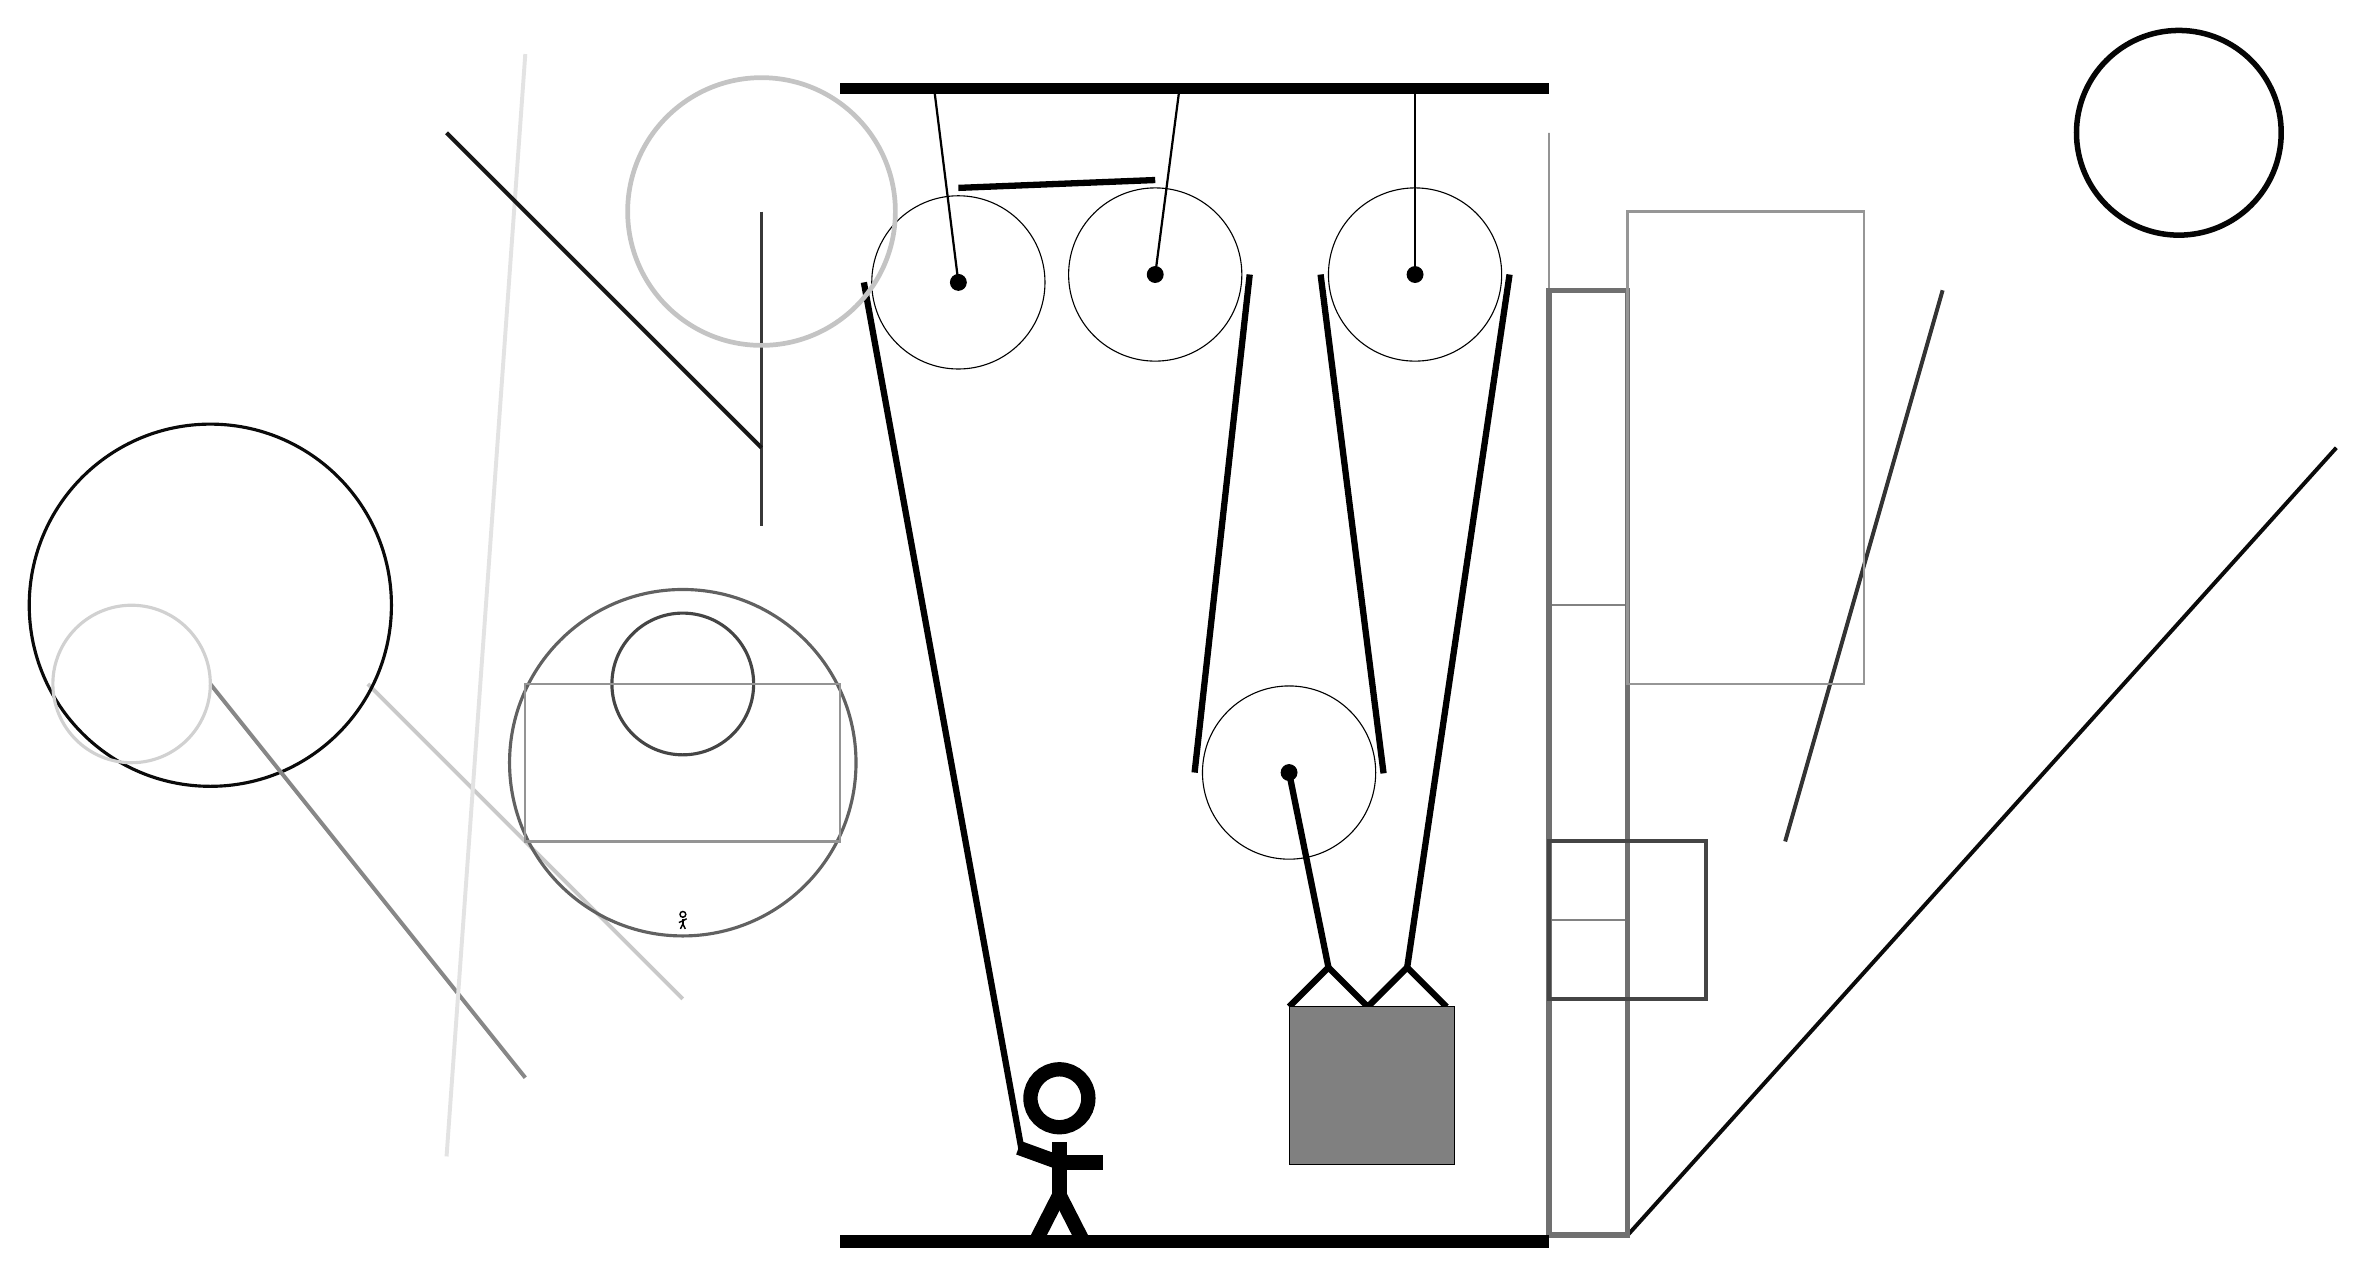
\begin{tikzpicture}
			%%%%% START %%%%%
			
			\draw[fill=black] (-3, 11.5) rectangle (6, 11.625);
			
			\draw (1, 9.2) circle (1.1);
			\draw[fill=black] (1, 9.2) circle (0.1);
			\draw[thick] (1, 9.2) -- (1.3, 11.5);
			
			\draw (4.3, 9.2) circle (1.1);
			\draw[fill=black] (4.3, 9.2) circle (0.1);
			\draw[thick] (4.3, 9.2) -- (4.3, 11.5);
			
			\draw (2.7, 2.875) circle (1.1);
			\draw[fill=black] (2.7, 2.875) circle (0.1);
			
			\draw[line width=0.8mm]  (2.7, -0.1) -- (3.2, 0.4) -- (3.7, -0.1) -- (4.2, 0.4) -- (4.7, -0.1);
			\draw[fill=black!50] (2.7, -0.1) rectangle (4.8, -2.1);
			
			\draw (-1.5, 9.1) circle (1.1);
			\draw[fill=black] (-1.5, 9.1) circle (0.1);
			\draw[thick] (-1.5, 9.1) -- (-1.8, 11.5);
			
			\draw[line width=0.8mm](-0.7, -1.9) --  (-2.7, 9.1);
			\centerarc[line width=0.8mm](-1.5, 9.1)(90:180:1.2000000000000002);
			\draw[line width=0.8mm](-1.5, 10.3) -- (1, 10.4);
			\centerarc[line width=0.8mm](1, 9.2)(0:90:1.2000000000000002);
			\draw[line width=0.8mm](2.2, 9.2) -- (1.5, 2.875);
			\centerarc[line width=0.8mm](2.7, 2.875)(180:370:1.2000000000000002);
			\draw[line width=0.8mm] (3.9, 2.865) -- (3.1, 9.2);
			\centerarc[line width=0.8mm](4.3, 9.2)(0:180:1.2000000000000002);
			\draw[line width=0.8mm](4.2, 0.4) -- (5.5, 9.2);
			\draw[line width=0.8mm] (3.2, 0.4) -- (2.7, 2.875);
			
			\node at (-0.2, -2) {\Strichmaxerl[10][-20][0]};
			
			\draw[line width=0.4mm, color=black!47] (7, 2) rectangle (7, 3);
			
			\draw[line width=0.5mm, color=black!21](-5, 0) -- (-9, 4);
			\draw [line width=0.4mm, color=black!96](-11, 5) circle (2.3);
			\draw[line width=0.3mm, color=black!42] (6, 11) rectangle (6, -2);
			
			\draw [line width=0.4mm, color=black!62](-5, 3) circle (2.2);
			\draw[line width=0.5mm, color=black!47](-7, -1) -- (-11, 4);
			\draw [line width=0.7mm, color=black!98](14, 11) circle (1.3);
			\draw[line width=0.5mm, color=black!78](-4, 10) -- (-4, 6);
			\draw[line width=0.5mm, color=black!11](-7, 12) -- (-8, -2);
			\draw[line width=0.5mm, color=black!96](7, -3) -- (16, 7);
			\draw [line width=0.6mm, color=black!23](-4, 10) circle (1.7);
			
			\draw[line width=0.5mm, color=black!91](-4, 7) -- (-8, 11);
			\draw [line width=0.4mm, color=black!73](-5, 4) circle (0.9);
			\draw[line width=0.2mm, color=black!49] (7, 1) rectangle (6, 5);
			\draw[line width=0.5mm, color=black!80](9, 2) -- (11, 9);
			\node[line width=0.4mm, color=black!99] at (-5, 1) {\Strichmaxerl[1][23][29]};
			
			\draw[line width=0.7mm, color=black!56] (7, -3) rectangle (6, 9);
			\draw[line width=0.3mm, color=black!41] (7, 10) rectangle (10, 4);
			\draw[line width=0.5mm, color=black!73] (8, 0) rectangle (6, 2);
			\draw [line width=0.4mm, color=black!18](-12, 4) circle (1.0);
			\draw[line width=0.3mm, color=black!42] (-3, 4) rectangle (-7, 2);
			
			\draw[fill=black] (-3, -3) rectangle (6, -3.15);
			
			%%%%% END %%%%%
		\end{tikzpicture}
	\end{figure}	
\end{document}